\documentclass[letter,12pt]{article}
\usepackage[paperheight=27.94cm,paperwidth=21.59cm,bindingoffset=0in,left=3cm,right=2.0cm, top=3.5cm,bottom=2.5cm, headheight=200pt, headsep=1.0\baselineskip]{geometry}
\usepackage{graphicx,lastpage}
\usepackage{upgreek}
\usepackage{censor}
\usepackage[spanish,es-tabla]{babel}
\usepackage{pdfpages}
\usepackage{tabularx}
\usepackage{graphicx}
\usepackage{adjustbox}
\usepackage{xcolor}
\usepackage{colortbl}
\usepackage{rotating}
\usepackage{multirow}
\usepackage[utf8]{inputenc}
\usepackage{float}
\usepackage{hyperref}

\renewcommand{\tablename}{Tabla}
\usepackage{fancyhdr}
\pagestyle{fancy}


%
\begin{document}
%
   \title{\Huge{Informe Laboratorio 5}}

   \author{\textbf{Sección 1} \\  \\Kevin Muñoz \\ kevin.munoz\_a@mail.udp.cl}
          
   \date{Junio de 2023}

   \maketitle
   
   \tableofcontents
 
  \newpage
  

\section{Descripción de actividades}
Para este último laboratorio, nuestro informante ya sabe que puede establecer un medio seguro sin un intercambio previo de una contraseña, gracias al protocolo diffie-hellman. El problema es que ahora no sabe si confiar en el equipo con el cual establezca comunicación, ya que las credenciales de usuario pueden haber sido divulgadas por algún soplón.\\

Para el presente laboratorio deberá:

\begin{itemize}
    \item Crear 4 contenedores en Docker, donde cada uno tendrá el siguiente SO:
        Ubuntu 14.10, Ubuntu 16.10, Ubuntu 18.10 y Ubuntu 20.10, a los cuales llamaremos C1,C2,C3,C4/S1 respectivamente.
        
    \item Para cada uno de ellos, deberá instalar la última versión, disponible en sus repositorios, del cliente y servidor openssh.

    \item En S1 deberá crear el usuario test con contraseña test, para acceder a él desde los otros contenedores.
    
    \item En total serán 4 escenarios, donde cada uno corresponderá a los siguientes equipos:
    \begin{itemize}
        \item C1 $\rightarrow$ S1
        \item C2 $\rightarrow$ S1
        \item C3 $\rightarrow$ S1
        \item C4 $\rightarrow$ S1
    \end{itemize}
\end{itemize}

Pasos:

\begin{enumerate}
\item Para cada uno de los 4 escenarios, solo deberá establecer la conexión y no realizar ningún otro comando que pueda generar tráfico (como muestra la Figura). Deberá capturar el tráfico de red generado y analizar el patrón de tráfico generado por cada cliente. De esta forma podrá obtener una huella digital para cada cliente a partir de su tráfico.\\

Indique el tamaño de los paquetes del flujo generados por el cliente y el contenido asociado a cada uno de ellos. Luego, indique qué información distinta contiene el escenario siguiente (diff incremental). El objetivo de esta tarea es identificar claramente los cambios entre las distintas versiones de ssh.

\newpage

\item Para poder identificar que el usuario efectivamente es el informante, éste utilizará una versión única de cliente. ¿Con qué cliente SSH se habrá generado el siguiente tráfico?

\begin{figure}[H]
    \centering
    \includegraphics[width=17.5cm]{Desarrollo/trafico.png}
    \caption{Tráfico generado del informante}
    \label{fig:ASCII}
\end{figure}

Replique este tráfico generado en la imagen. Debe generar el tráfico con la misma versión resaltada en azul.

\newpage

\item Para que el informante esté seguro de nuestra identidad, nos pide que el patrón del tráfico de nuestro server también sea modificado, hasta que el Key Exchange Init del server sea menor a 300 bytes. Indique qué pasos realizó para lograr esto.

\begin{figure}[H]
    \centering
    \includegraphics[width=17.5cm]{Desarrollo/exchange.png}
    \caption{Captura del Key Exchange}
    \label{fig:ASCII}
\end{figure}

\end{enumerate}


\section{Desarrollo (Parte 1)}

\subsection{Códigos de cada Dockerfile}
\subsubsection{S1}
Para este caso el codigo de C4 tambien correspondera al de S1.
    \begin{figure}[H]
        \centering
        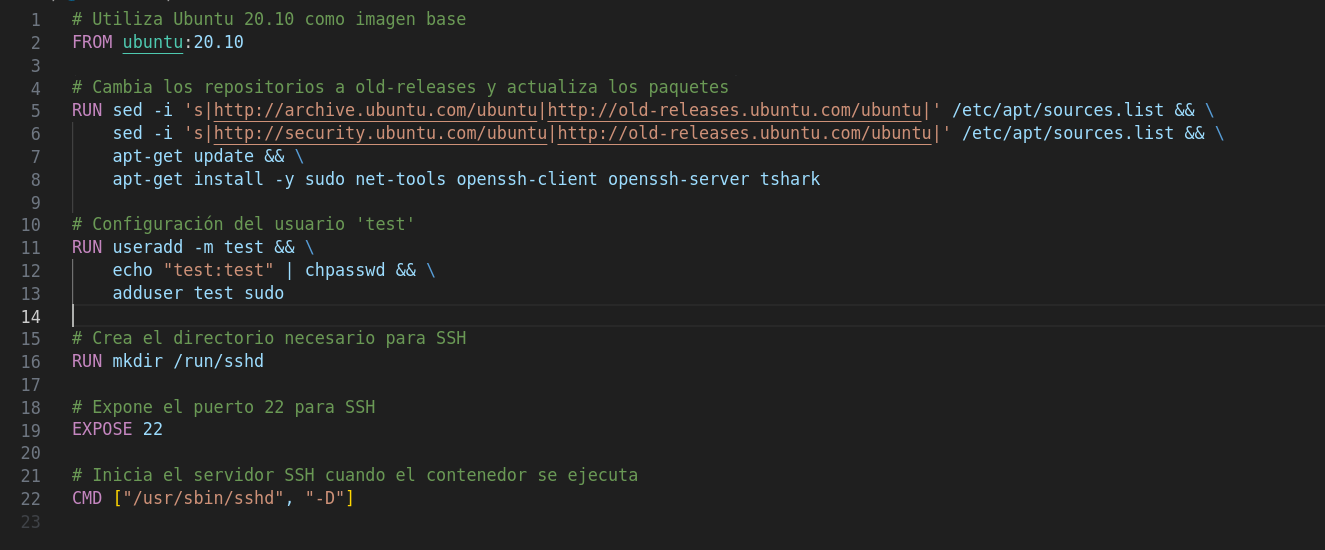
\includegraphics[width=1\textwidth]{img/s1_c4.png}
        \caption{Codigo dockerfile s1 y c4}
    \end{figure}
\subsubsection{C1}
    \begin{figure}[H]
        \centering
        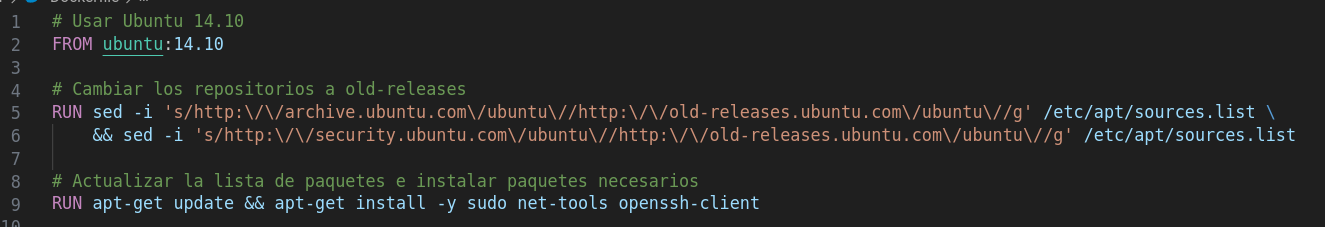
\includegraphics[width=1\textwidth]{img/c1_codigo.png}
        \caption{Codigo dockerfile c1}
    \end{figure}
Este Dockerfile crea una imagen de Docker basada en Ubuntu 14.10, cambia los repositorios de paquetes a versiones antiguas y luego instala herramientas esenciales como sudo, net-tools y openssh-client.

\subsubsection{C2}
    \begin{figure}[H]
        \centering
        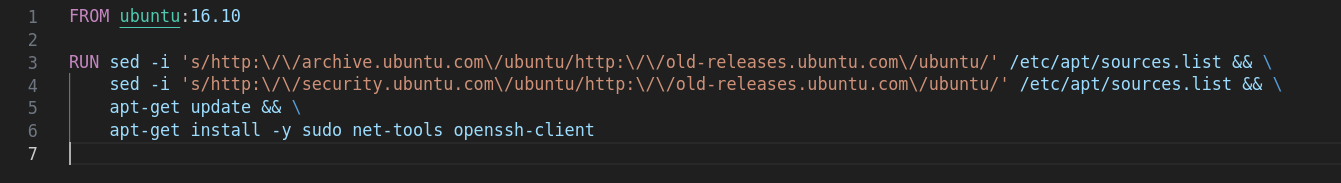
\includegraphics[width=1\textwidth]{img/c2.png}
        \caption{Codigo dockerfile c2}
    \end{figure}
Este Dockerfile crea una imagen de Docker basada en ubuntu 16.10, cambia los reposi-
torios de paquetes a versiones antiguas y luego instala herramientas esenciales como sudo,
net-tools y openssh-client.
5

\subsubsection{C3}
    \begin{figure}[H]
        \centering
        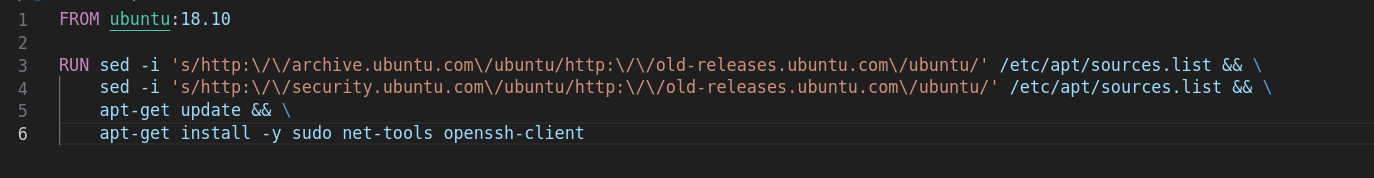
\includegraphics[width=1\textwidth]{img/c3.png}
        \caption{Codigo dockerfile c3}
    \end{figure}
Este Dockerfile crea una imagen de Docker basada en ubuntu 18.10, cambia los reposi-
torios de paquetes a versiones antiguas y luego instala herramientas esenciales como sudo,
net-tools y openssh-client.
5

\subsubsection{C4}
    \begin{figure}[H]
        \centering
        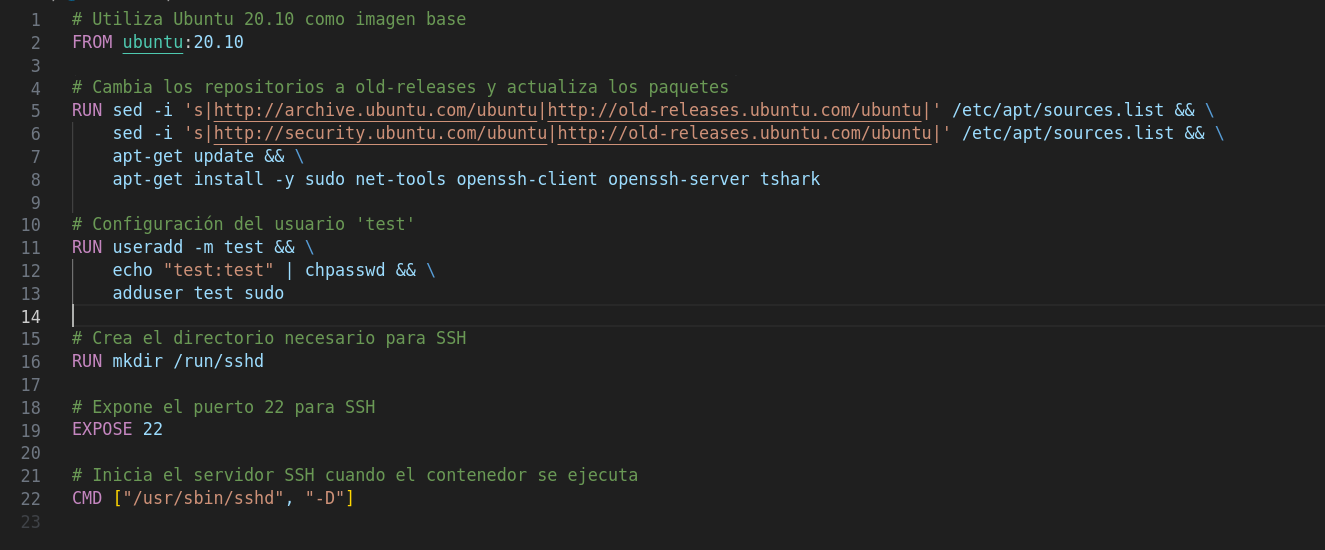
\includegraphics[width=1\textwidth]{img/s1_c4.png}
        \caption{Codigo dockerfile s1 y c4}
    \end{figure}
Base en Ubuntu 20.10: Usa Ubuntu 20.10 como imagen base.

Cambio de Repositorios y Actualización de Paquetes: Modifica los repositorios de paquetes a old-releases.ubuntu.com, y luego actualiza e instala paquetes esenciales, incluyendo sudo, net-tools, openssh-client, openssh-server y tshark.

Configuración de Usuario test: Crea un usuario llamado test con contraseña test, y lo añade al grupo sudo.

Preparación para SSH: Crea un directorio necesario para el servicio SSH.

Exposición del Puerto 22: Expone el puerto 22 para conexiones SSH.

Inicio del Servidor SSH: Configura el contenedor para iniciar el servidor SSH cuando se ejecuta.
\subsection{Creación de las credenciales para S1}

Las credenciales se establecen al inicio del Dockerfile C4, mediante los siguientes comandos: se crea el usuario test con un directorio home, se establece su contraseña como test, y se le añade al grupo sudo. Esto se realiza con la instrucción: RUN useradd -m test \&\& echo "test:test" | chpasswd \&\& adduser test sudo.

    \begin{figure}[H]
        \centering
        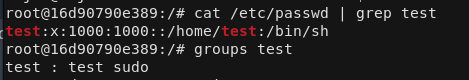
\includegraphics[width=1\textwidth]{img/credenciales_s1.png}    
        \caption{Credenciales S1}
    \end{figure}

como se puede apreciar las credenciales para s1 se crearon correctamente verficando el grupo correspondiente dentro del dockerfile C4.
\subsection{Tráfico generado por C1 (detallado)}
El primer paso en el proceso de interconexión de contenedores Docker involucra la preparación del contenedor que actuará como servidor SSH, identificado como S1. Dentro de este contenedor, el servicio SSH se inicia ejecutando service ssh start. Este paso es crucial, ya que prepara el contenedor S1 para aceptar conexiones entrantes. Después de iniciar el servicio SSH, es necesario obtener la dirección IP del contenedor. Esto se logra mediante el comando hostname -I. La dirección IP obtenida será utilizada por el contenedor cliente para establecer la conexión SSH.
    \begin{figure}[H]
        \centering
        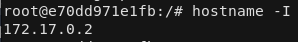
\includegraphics[width=1\textwidth]{img/direccio_ip_s1.png}    
        \caption{Obtencion direccion ip}
    \end{figure}
Una vez que el contenedor S1 está configurado y su dirección IP conocida, el foco se traslada al contenedor C1, que funcionará como cliente SSH. Desde C1, se inicia una conexión SSH hacia S1 utilizando el comando ssh test@ip\_de\_S1, donde ip\_de\_S1 es la dirección IP del contenedor S1. Durante este proceso, el usuario debe autenticarse proporcionando la contraseña del usuario test. Este paso es esencial para la seguridad de la conexión, ya que verifica la identidad del usuario antes de permitir el acceso al contenedor servidor.

    \begin{figure}[H]
        \centering
        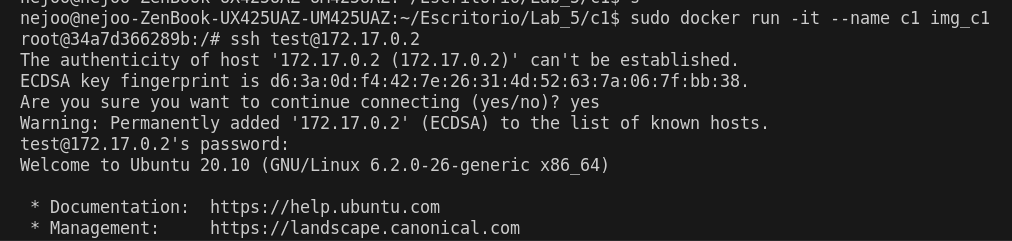
\includegraphics[width=1\textwidth]{img/conecion_c1.png}    
        \caption{Conexión c1}
    \end{figure}

    Paralelamente a la conexión SSH, se utiliza Wireshark para capturar y analizar el tráfico de red entre los contenedores. Este análisis revela varios aspectos clave de la comunicación SSH. Primero, se observa que las versiones de OpenSSH difieren entre los contenedores, siendo 6.6 en el cliente (C1) y 8.3 en el servidor (S1). Durante la fase de establecimiento de la conexión, se identifica un intercambio de claves siguiendo el protocolo Diffie-Hellman. Este intercambio permite que ambos contenedores acuerden una clave secreta para sus comunicaciones sin la necesidad de transmitirla a través del canal. Los primeros paquetes en este intercambio especifican los algoritmos soportados por cada lado, permitiendo así seleccionar un algoritmo común para el cifrado de las comunicaciones subsecuentes.

    \begin{figure}[H]
        \centering
        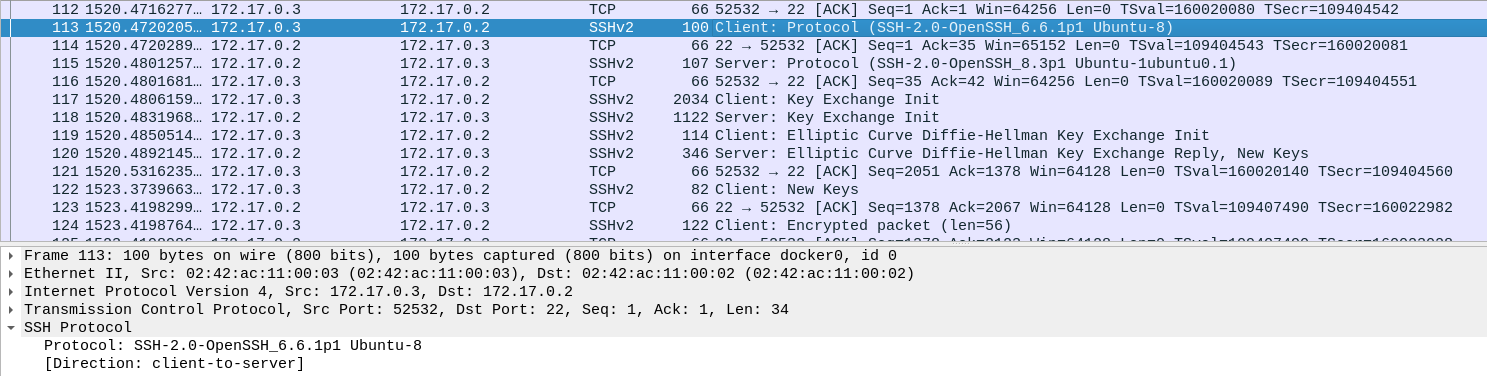
\includegraphics[width=1\textwidth]{img/captura_wire.png}    
        \caption{Captura de Wireshark}
    \end{figure}
Además, se destaca que el tamaño de los paquetes durante esta comunicación varía, oscilando generalmente entre 60 y 200 bytes. Sin embargo, los paquetes relacionados con el detalle de los algoritmos de cifrado son significativamente más grandes, con el paquete del cliente conteniendo aproximadamente 2034 bytes y el del servidor alrededor de 1122 bytes. Estos detalles son esenciales para comprender la naturaleza y la seguridad de la comunicación SSH entre los contenedores Docker.
    \begin{figure}[H]
        \centering
        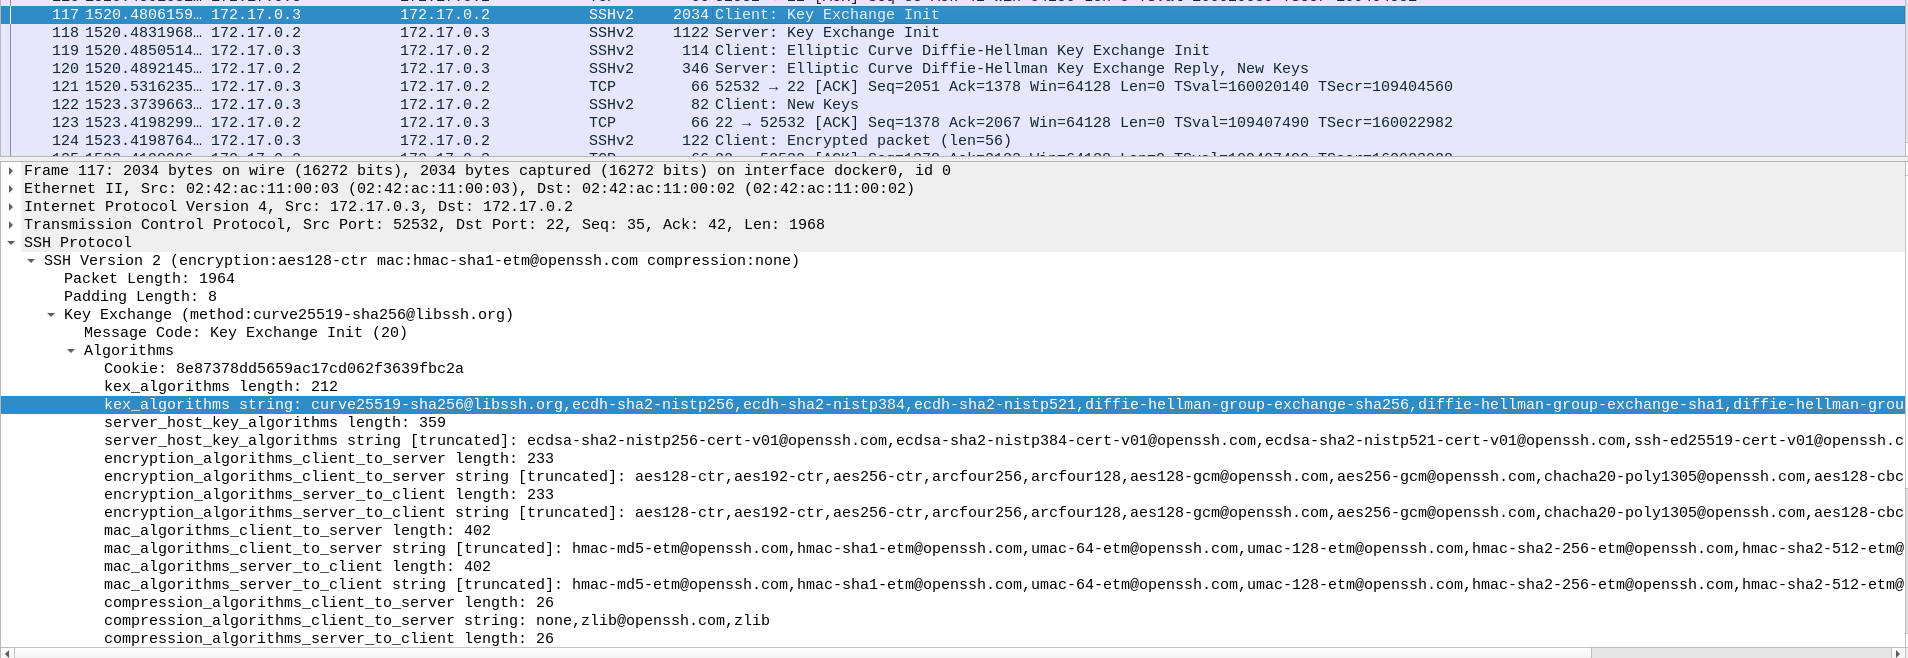
\includegraphics[width=1\textwidth]{img/algoritmos.png}    
        \caption{Captura de Wireshark}
    \end{figure}
\subsection{Tráfico generado por C2 (detallado)}
El proceso de interconexión de contenedores Docker mediante SSH es el mismo que el anterior, comienza con la configuración del contenedor servidor, S1. Primero, se activa el servicio SSH dentro de S1 utilizando service ssh start, preparándolo para recibir conexiones. Luego, se obtiene la dirección IP de S1 mediante hostname -I, la cual es necesaria para que el contenedor cliente, C2, se conecte a él. Después, en C2, se establece una conexión SSH hacia S1 con el comando ssh test@ip\_de\_S1, usando la dirección IP de S1. Durante este proceso, es crucial autenticarse con la contraseña del usuario test para garantizar la seguridad y la verificación de identidad antes de acceder al contenedor servidor.
    \begin{figure}[H]
        \centering
        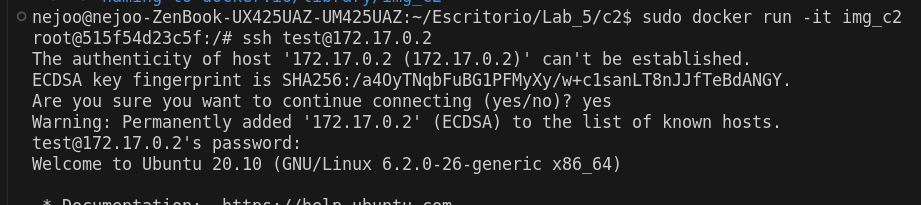
\includegraphics[width=1\textwidth]{img/conexion_c2.png}    
        \caption{Conexion C2 hacia S1}
    \end{figure}
    
Durante la captura de tráfico SSH con el cliente C2, se observaron detalles específicos en la comunicación con el servidor S1. El cliente C2 utilizaba la versión 7.3 de OpenSSH, y el análisis del tráfico reveló que el paquete que detalla los algoritmos soportados por este cliente tenía un tamaño de 1498 bytes, indicativo de los algoritmos de cifrado y otros mecanismos de seguridad que puede emplear. En contraste, el paquete del servidor S1 que responde con los algoritmos soportados por el servidor mantuvo un tamaño constante de 1122 bytes. Estos detalles son críticos en el proceso de establecimiento de la conexión SSH, pues aseguran que tanto el cliente como el servidor acuerden un conjunto de algoritmos compatibles y seguros para la comunicación cifrada, reflejando así las variaciones en la configuración de seguridad y los algoritmos disponibles entre diferentes clientes.
    \begin{figure}[H]
        \centering
        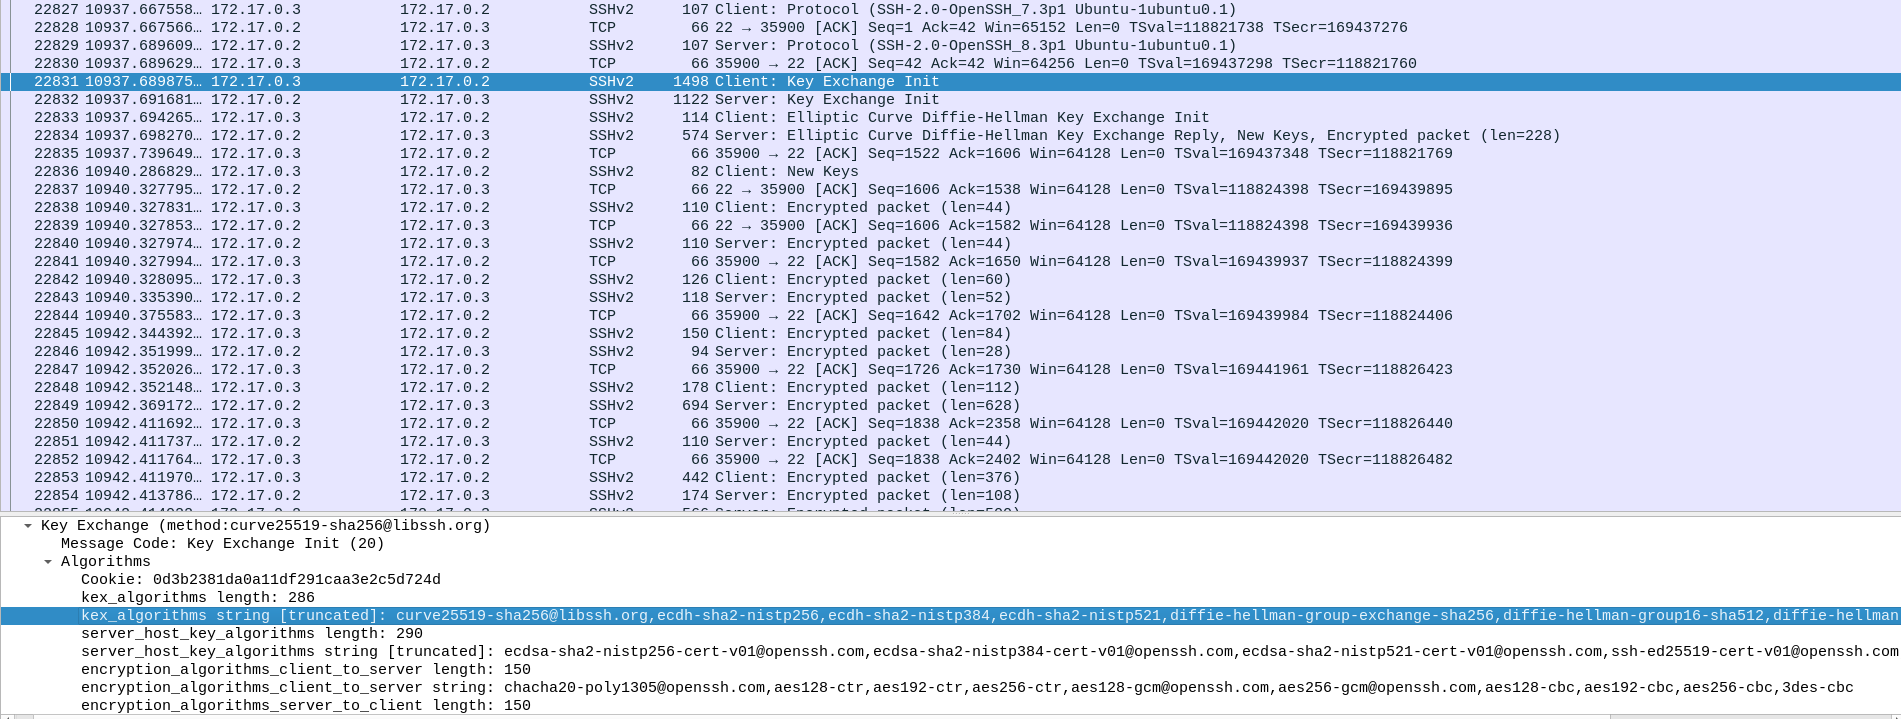
\includegraphics[width=1\textwidth]{img/captura_c2.png}    
        \caption{Captura conexion c2 hacia s1}
    \end{figure}
\subsection{Tráfico generado por C3 (detallado)}
El proceso de interconexión de contenedores Docker mediante SSH es el mismo que el anterior, comienza con la configuración del contenedor servidor, S1. Primero, se activa el servicio SSH dentro de S1 utilizando service ssh start, preparándolo para recibir conexiones. Luego, se obtiene la dirección IP de S1 mediante hostname -I, la cual es necesaria para que el contenedor cliente, C3, se conecte a él. Después, en C3, se establece una conexión SSH hacia S1 con el comando ssh test@ip\_de\_S1, usando la dirección IP de S1. Durante este proceso, es crucial autentificarse con la contraseña del usuario test para garantizar la seguridad y la verificación de identidad antes de acceder al contenedor servidor.
    \begin{figure}[H]
        \centering
        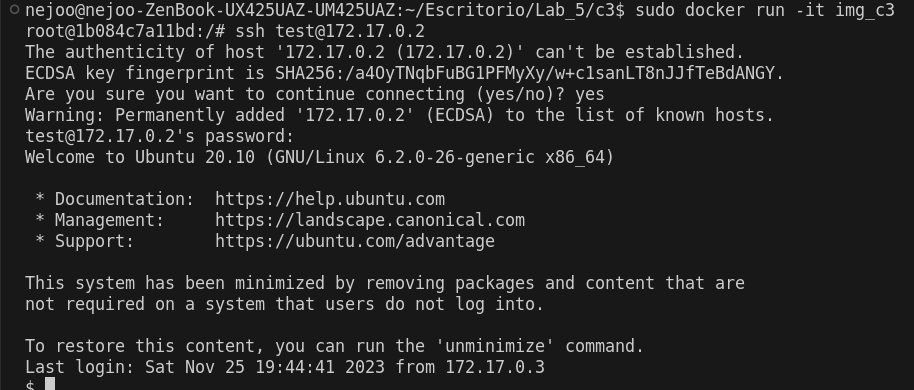
\includegraphics[width=1\textwidth]{img/creacion_c3.png}    
        \caption{Conexion C3 a s1}
    \end{figure}

análisis de tráfico SSH para el cliente C3, se observaron ciertos detalles específicos que reflejan características únicas de esta conexión. El cliente C3 estaba utilizando la versión 7.7 de OpenSSH, una información relevante para entender el contexto de la comunicación y las capacidades de cifrado que ofrece esta versión específica del software.

El análisis del tráfico reveló que el tamaño del paquete que detalla los algoritmos soportados por el cliente C3 era de 1426 bytes. Este tamaño es indicativo de los algoritmos de cifrado, intercambio de claves y otros mecanismos de seguridad que el cliente está dispuesto y capacitado para utilizar durante la sesión SSH. El hecho de que el paquete tenga un tamaño de 1426 bytes sugiere un conjunto específico de algoritmos y configuraciones de seguridad que el cliente C3 está empleando.

    \begin{figure}[H]
        \centering
        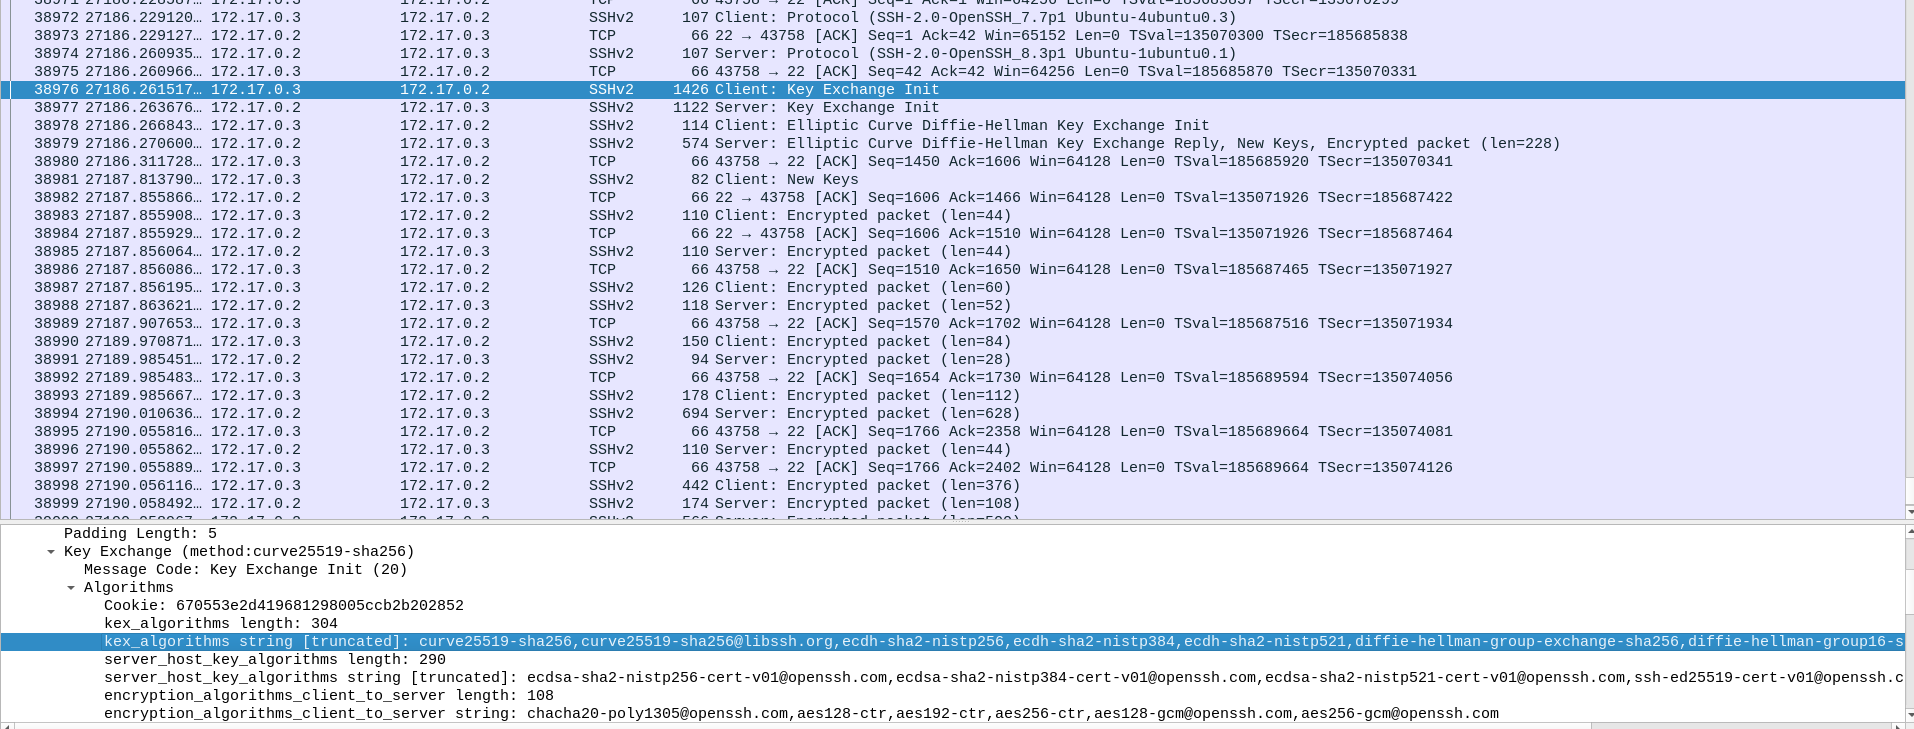
\includegraphics[width=1\textwidth]{img/captura_c3.png}    
        \caption{Captura wireshark conexion C3 a s1}
    \end{figure}


\subsection{Tráfico generado por C4 (4 (iface lo) (detallado)}

Para capturar el tráfico SSH dentro del contenedor C4, se empleó un método específico que implicó la modificación de ciertas variables y la concesión de privilegios de administrador. Esto se logró iniciando el contenedor con el comando sudo docker run -it --cap-add=NET\_RAW --cap-add=NET\_ADMIN --privileged c4. Esta configuración era necesaria para permitir la captura de datos desde dentro del contenedor utilizando herramientas como tshark.

El proceso de captura y análisis se llevó a cabo utilizando dos terminales. La primera terminal se dedicó a realizar la captura de tráfico, iniciada con el comando mencionado anteriormente. La otra terminales se abrieron utilizando sudo docker exec -it 102b81a8e50d bash, una vez dentro de la bash se procedio a iniciar captura con tshark.



\begin{figure}[H]
        \centering
        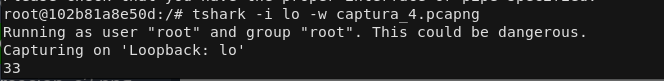
\includegraphics[width=1\textwidth]{img/paquetes_c4.png}    
        \caption{Captura tshark conexion C4 a C4}
    \end{figure}

Para establecer la conexión SSH, primero se inició el servidor en una de las terminales, y luego, en la terminal del cliente, se utilizó el comando ssh test@localhost para realizar una conexión SSH de vuelta al mismo contenedor. Justo antes de iniciar esta conexión, se comenzó la captura de tráfico en la primera terminal.
\begin{figure}[H]
        \centering
        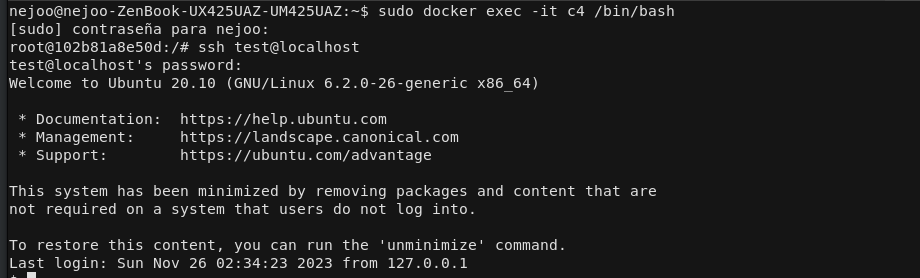
\includegraphics[width=1\textwidth]{img/conexion_c4.png}    
        \caption{Conexion C4 a C4}
    \end{figure}
En el análisis de la captura, se observó que tanto el cliente como el servidor dentro de C4 utilizaban la misma versión de OpenSSH, que era la 8.3. Este resultado era esperado, ya que ambos procesos, cliente y servidor, se ejecutaban dentro del mismo contenedor y, por lo tanto, compartían la misma configuración de software. Sin embargo, un detalle interesante fue que, a pesar de que los paquetes que detallan los algoritmos contenían la misma información (dado que cliente y servidor son el mismo entorno), sus tamaños eran distintos en este caso 1426 bytes.
\begin{figure}[H]
        \centering
        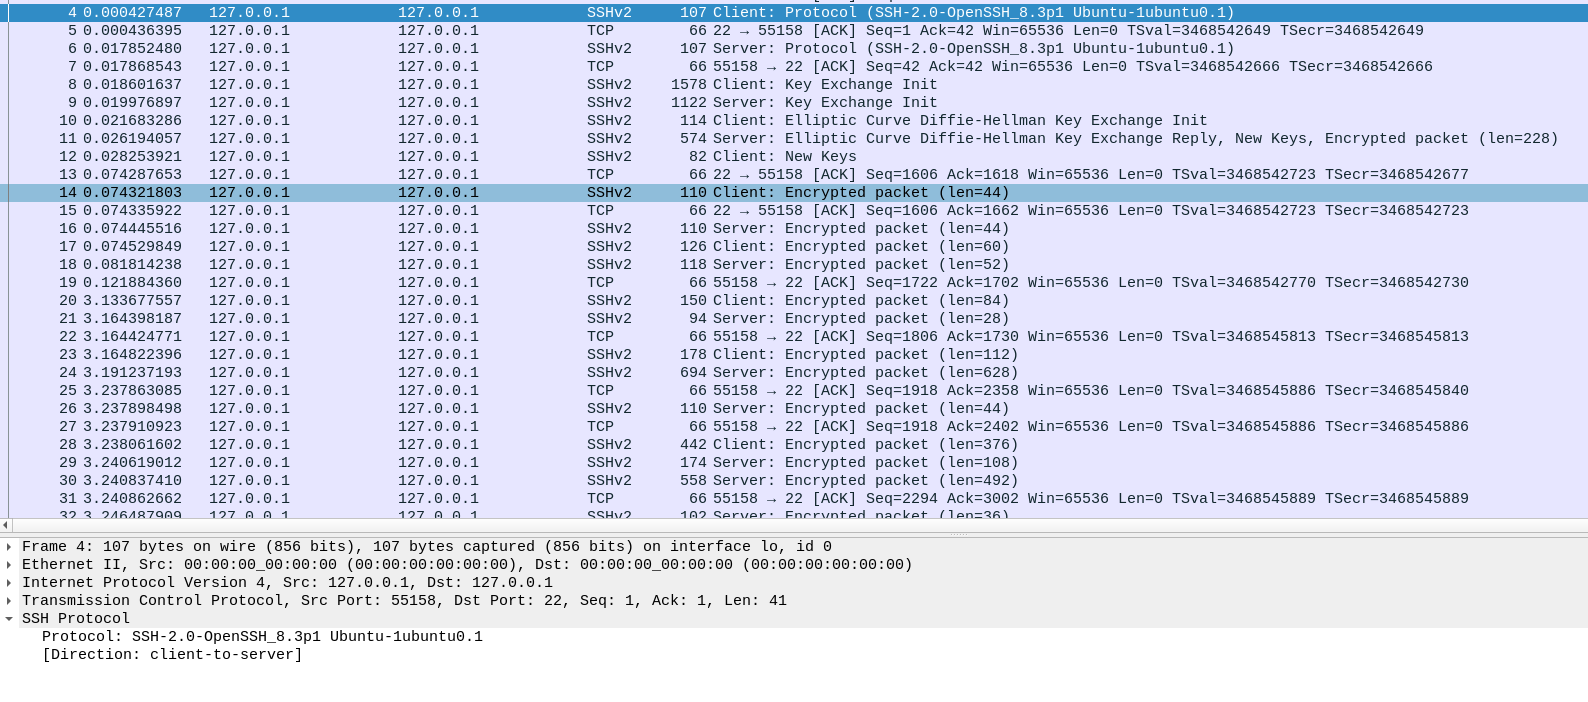
\includegraphics[width=1\textwidth]{img/wireshar_c4.png}    
        \caption{Captura wireshark conexion C4 a C4}
    \end{figure}
\subsection{Diferencia entre C1 y C2}
Las diferencias clave entre los clientes C1 y C2 en el contexto de sus sesiones SSH radican en las versiones de OpenSSH y el tamaño de los paquetes de algoritmos utilizados. Mientras que la versión específica de OpenSSH en C1 no se detalla, en C2 se emplea la versión 7.3. Esta diferencia en las versiones sugiere variaciones en las capacidades de seguridad y los algoritmos soportados. Además, el tamaño del paquete de algoritmos es notablemente mayor en C1, con aproximadamente 2034 bytes, en comparación con los 1498 bytes en C2, lo que indica una lista más extensa de algoritmos soportados por C1. Estas diferencias pueden tener implicaciones significativas en términos de compatibilidad, seguridad y la eficacia de las comunicaciones cifradas entre los clientes y el servidor.
\subsection{Diferencia entre C2 y C3}
En la comparación entre los clientes C2 y C3 en sus respectivas sesiones SSH, las diferencias principales se centran en las versiones de OpenSSH y el tamaño de los paquetes de algoritmos. El cliente C2 utiliza OpenSSH versión 7.3, mientras que C3 opera con la versión 7.7. Esta variación en las versiones indica una posible diferencia en las capacidades de seguridad, rendimiento y los algoritmos disponibles entre ambos clientes, dado que las versiones más recientes suelen incorporar mejoras y correcciones. Además, el tamaño del paquete de algoritmos en C2 es de 1498 bytes, mientras que en C3 es ligeramente menor, con 1426 bytes. Aunque ambos tamaños son similares, sugiriendo una lista de algoritmos soportados parecida, la diferencia de tamaño podría reflejar ligeras variaciones en los algoritmos específicos o sus configuraciones entre estas dos versiones. Estas diferencias, aunque sutiles, pueden influir en la seguridad y la eficiencia de las comunicaciones SSH entre los clientes y el servidor.
\subsection{Diferencia entre C3 y C4}
Las diferencias entre los clientes C3 y C4 en sus sesiones SSH son principalmente la versión de OpenSSH y la configuración de la sesión SSH. C3 utiliza OpenSSH versión 7.7, mientras que C4, que actúa simultáneamente como cliente y servidor en el mismo contenedor, opera con la versión 8.3. Esta variación en las versiones de OpenSSH sugiere diferencias en las capacidades de seguridad y en la selección de algoritmos. Además, la configuración única de C4, donde la conexión SSH se realiza internamente (ssh test@localhost), contrasta con la configuración más convencional de C3 y podría influir en cómo se manejan y negocian los paquetes de algoritmos, incluso cuando se espera que el cliente y el servidor, siendo el mismo sistema, compartan configuraciones idénticas.
\section{Desarrollo (Parte 2)}

\subsection{Identificación del cliente ssh}
Podemos determinar que el cliente en cuestión es C4 basándonos en el tamaño específico del paquete de Intercambio de Claves de Elgamal (KEI, por sus siglas en inglés) emitido por el cliente, que es de 1578 bytes. Este tamaño coincide exactamente con el observado en la captura de tráfico realizada de C4 a sí mismo, tal como se muestra en la figura siguiente. Esta coincidencia en el tamaño del paquete KEI nos permite concluir que la versión de OpenSSH utilizada es la 8.3, que es la correspondiente a la distribución de Ubuntu 20.10. Esta identificación precisa del cliente a través del análisis de los detalles de la captura de tráfico es un claro indicador de la versión específica de OpenSSH en uso.
\begin{figure}[H]
        \centering
        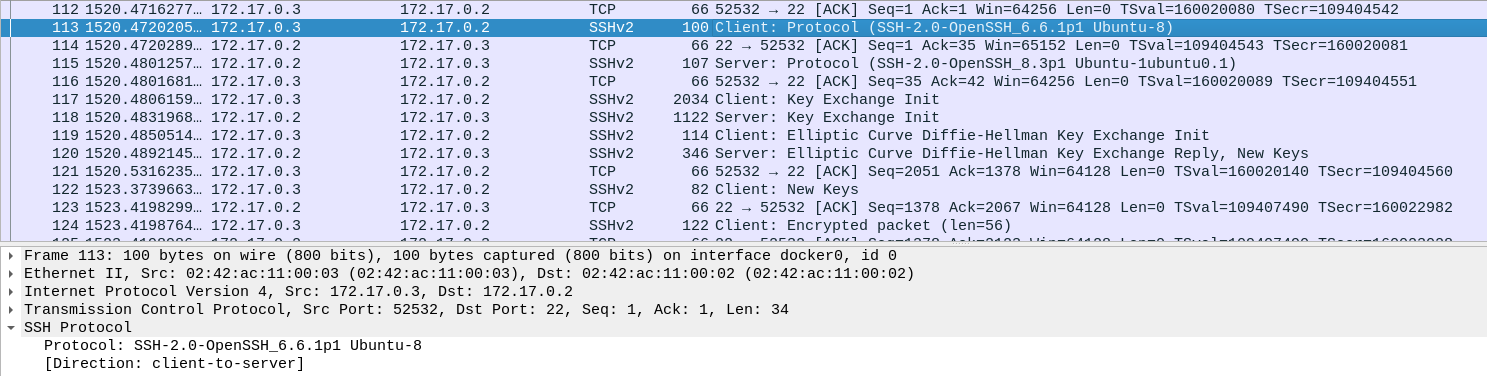
\includegraphics[width=1\textwidth]{img/captura_wire.png}  
        \caption{Captura wireshark version cliente}
    \end{figure}
\subsection{Replicación de tráfico (paso por paso)}
Para replicar el signo de interrogación observado en el tráfico SSH, es necesario recompilar OpenSSH. Utilizaremos para ello la versión portable de OpenSSH disponible en el repositorio de GitHub en https://github.com/openssh/openssh-portable. Para llevar a cabo esta tarea, crearemos una versión modificada de nuestro contenedor C4, que llamaremos C4 mod, utilizando el siguiente Dockerfile:
\begin{figure}[H]
        \centering
        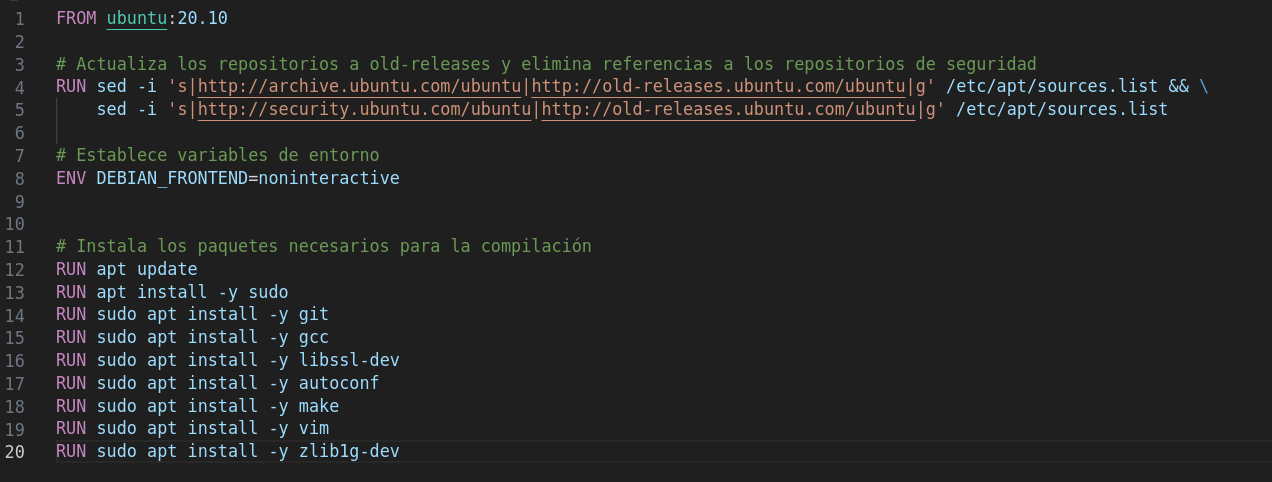
\includegraphics[width=1\textwidth]{img/docker_c4_mod.png}  
        \caption{dockerfile para modficar}
    \end{figure}
Este Dockerfile instala la misma versión de Ubuntu que C4, además de varios programas necesarios para la compilación. Inicializaremos este contenedor de la misma manera que C4 y clonaremos el repositorio de GitHub con git clone. Una vez clonado el repositorio, modificaremos el archivo version.h, que contiene los detalles de la versión del software. En este archivo, cambiaremos el número de versión por un signo de interrogación y eliminaremos la variable SSH\_PORTABLE.
\begin{figure}[H]
        \centering
        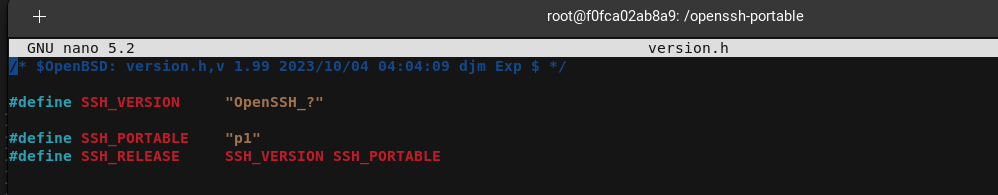
\includegraphics[width=1\textwidth]{img/nano_c4_new.png}  
        \caption{Modificando parametros}
    \end{figure}
Una vez finalizada la instalación, nos conectaremos a nuestro contenedor C4 mod y capturaremos el tráfico como ya lo realizamos antes. Podremos observar que la versión aparece como un signo de interrogación y que el tamaño del resto de los paquetes coincide con lo observado anteriormente. Esta modificación nos permite replicar con precisión el aspecto específico del tráfico SSH que estamos investigando.
\begin{figure}[H]
        \centering
        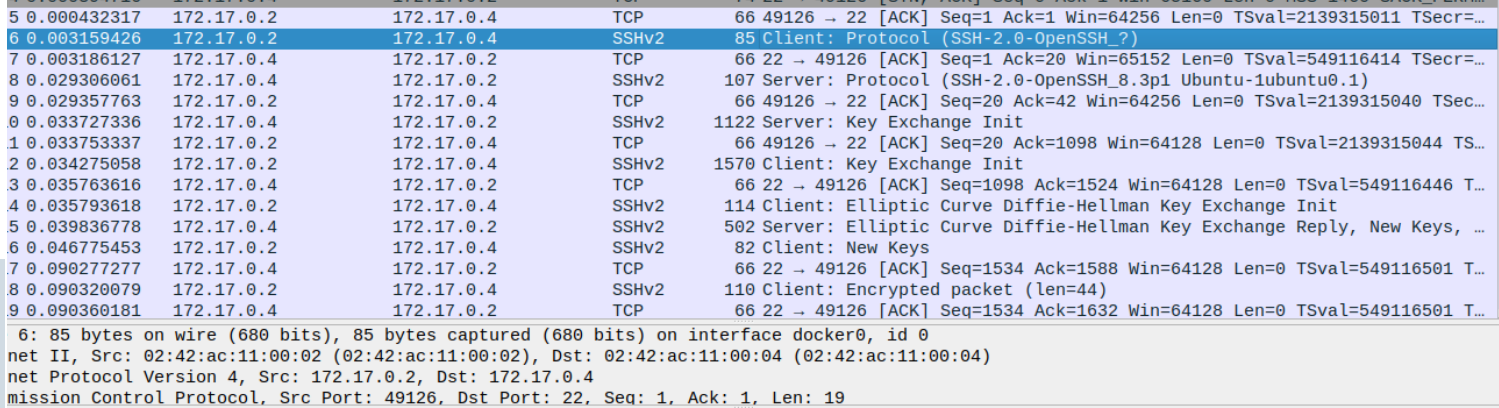
\includegraphics[width=1\textwidth]{img/docker__c4_mode.png}  
        \caption{Captura wireshark versionmodificada}
    \end{figure}
\section{Desarrollo (Parte 3)}

\subsection{Replicación de tráfico (paso por paso)}
Primero, construye el contenedor C5 utilizando el mismo Dockerfile que para C4. Esto garantiza que ambos contenedores compartan una base común. Comienza ubicándote en el directorio donde está el Dockerfile. Luego, construye la imagen Docker como ya se hizo previamente. Después de construir la imagen, inicia el contenedor C5.\\

El siguiente paso implica configurar el servidor SSH en C5. Esto se hace editando el archivo sshd\_config, ubicado en /etc/ssh/. Para acceder a C5, usa docker exec -it C5 /bin/bash. Una vez dentro del contenedor, abre el archivo de configuración SSH con un editor, como nano /etc/ssh/sshd\_config. En este archivo, localiza las secciones para Ciphers, KexAlgorithms y MACs. Modifica estas líneas para incluir solo un algoritmo en cada categoría, lo que reducirá el tamaño del paquete de intercambio de claves. Guarda los cambios y reinicia el servicio SSH con service ssh restart.
\begin{figure}[H]
        \centering
        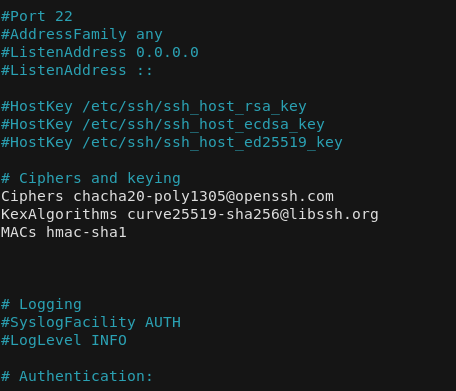
\includegraphics[width=1\textwidth]{img/modificacion.png}  
        \caption{Modificando de configuracion}
    \end{figure}
    
\begin{figure}[H]
        \centering
        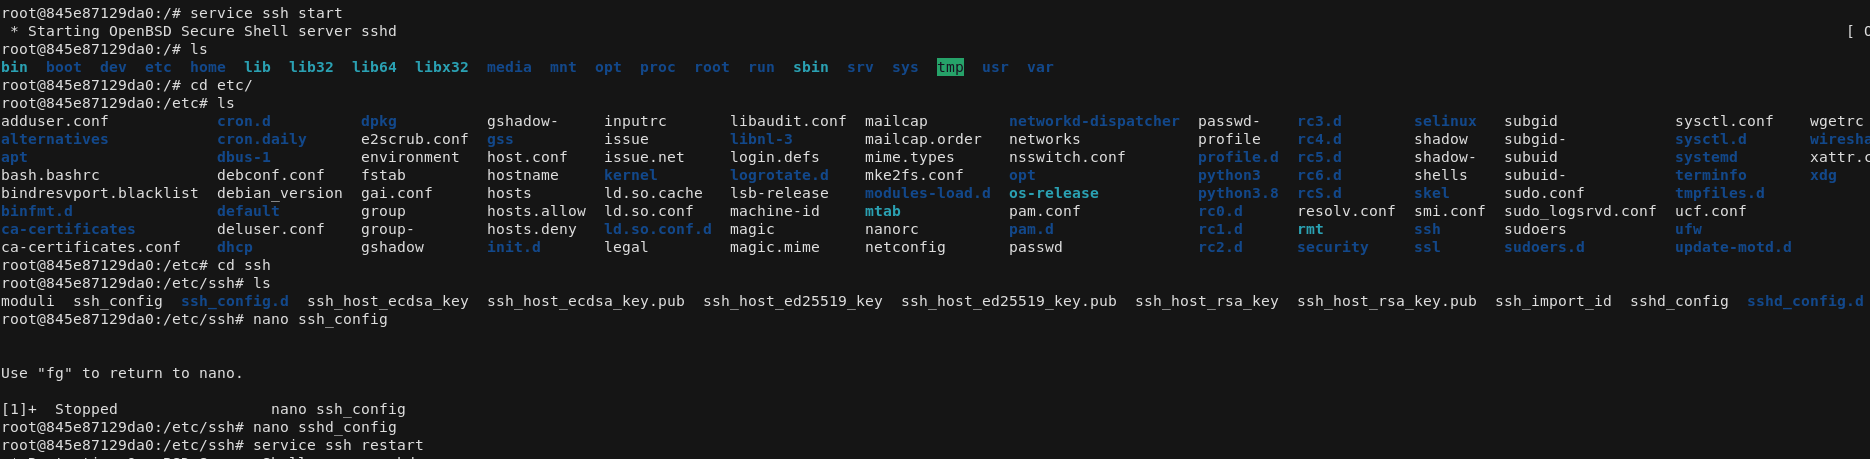
\includegraphics[width=1\textwidth]{img/restar.png}  
        \caption{Modificando ssh}
    \end{figure}

    \begin{figure}[H]
        \centering
        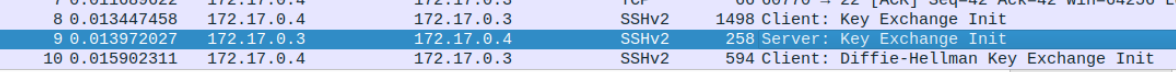
\includegraphics[width=1\textwidth]{img/final_paquete.png}  
        \caption{Paquete modificafo con menor tamaño}
    \end{figure}

    Finalmente, analiza el tráfico capturado para verificar el tamaño de los paquetes. Deberías notar que el tamaño del paquete es menor debido a la configuración de algoritmos más limitada en el servidor SSH de C5. Este análisis te ayudará a entender cómo las configuraciones específicas del servidor SSH afectan el tráfico y el tamaño de los paquetes en una sesión SSH. 
% Please add the following required packages to your document preamble:
%\begin{table}[htbp]
\newpage
\section*{Conclusiones y comentarios}
El informe revela cómo las distintas versiones de OpenSSH y las configuraciones de los contenedores afectan el tráfico SSH. Se destaca la importancia de los algoritmos de cifrado y la configuración del servidor en la determinación del tamaño y la estructura del tráfico SSH. Al modificar estas variables, se logra alterar el patrón de tráfico, lo que es crucial para propósitos de identificación y seguridad en comunicaciones cifradas. El laboratorio demuestra una metodología efectiva para el análisis y la manipulación del tráfico SSH, resaltando su relevancia en la seguridad de las redes y la comunicación de datos.
\end{document}
